\documentclass[conference]{IEEEtran}
\IEEEoverridecommandlockouts
\usepackage{cite}
\usepackage{amsmath,amssymb,amsfonts}
\usepackage{algorithm}
\usepackage{algorithmic}
\usepackage{graphicx}
\usepackage{textcomp}
\usepackage{xcolor}
\usepackage{booktabs}
\usepackage{url}
\newif\ifshowphotos
\showphotosfalse % set to \showphotostrue to include the two bench photographs
\usepackage{tikz}
\usetikzlibrary{shapes.geometric,arrows.meta,positioning,fit,backgrounds,calc}

\def\BibTeX{{\rm B\kern-.05em{\sc i\kern-.025em b}\kern-.08em
    T\kern-.1667em\lower.7ex\hbox{E}\kern-.125emX}}

\begin{document}

\title{Autonomous Predictive Drip Irrigation and Water Consumption\\
Monitoring System Using Hall Effect Sensor}

\author{
\IEEEauthorblockN{\small Harsh Singh}
\IEEEauthorblockA{\footnotesize School of Computer Science\\and Engineering\\Vellore Institute of Technology\\Vellore, India\\harsh.singh2023c@vitstudent.ac.in}
\and
\IEEEauthorblockN{\small Manya Shrivastava}
\IEEEauthorblockA{\footnotesize School of Computer Science\\and Engineering\\Vellore Institute of Technology\\Vellore, India\\manya.shrivastava2023@vitstudent.ac.in}
\and
\IEEEauthorblockN{\small A. Charanjith Reddy}
\IEEEauthorblockA{\footnotesize School of Computer Science\\and Engineering\\Vellore Institute of Technology\\Vellore, India\\charanjithreddy.a2023@vitstudent.ac.in}
\and
\IEEEauthorblockN{\small Naresh K}
\IEEEauthorblockA{\footnotesize School of Computer Science\\and Engineering\\Vellore Institute of Technology\\Vellore, India\\naresh.k@vit.ac.in}
}

\maketitle

\begin{abstract}
Smallholder drip irrigation can be made more water-efficient by combining
local soil-moisture sensing with a short-term rainfall forecast, so that
irrigation is withheld when rain is already expected. This paper reports
the design and bench-prototype implementation of such a system, built
around an ESP32 edge controller, a capacitive soil-moisture sensor, a
DHT11 temperature/humidity sensor, a Hall-effect turbine flow sensor for
volumetric water accounting, and a relay-driven pump/solenoid actuator.
The firmware combines a local soil-moisture threshold with a direct
HTTP call to an external weather-forecast API and withholds irrigation
when dry soil and a forecast rain probability above a configurable
threshold coincide. Two independent safety interlocks, a maximum pump
run-time and a no-flow-pulse fault, force the actuator off regardless of
the irrigation decision. The paper reports implementation status rather
than performance figures: the firmware source, a bench serial-monitor
log and photographs of the assembled hardware support the design, while
calibration accuracy, water savings, forecast-skip precision and relay
polarity remain to be validated. Each claim is classified by the
strength of its supporting evidence using a five-category scheme that
can be reused in other early-stage hardware projects.
\end{abstract}

\begin{IEEEkeywords}
predictive irrigation, soil moisture sensing, ESP32, Hall-effect flow sensor, IoT agriculture, evidentiary classification, prototype implementation
\end{IEEEkeywords}

\section{Introduction}

The majority of freshwater withdrawn from India's water resources comes from
the agricultural sector; national water management assessments have repeatedly
shown that both groundwater over-pumping and inefficient irrigation are major
structural threats to India's long-term food and water security
\cite{niti2019cwmi,fao2024aquastat}. The continued decline in groundwater
levels across northern India, as shown by satellite gravimetry data, further
supports this finding \cite{rodell2009groundwater}. Irrigation inefficiencies
are primarily caused by a lack of predictive decision-making using weather
forecasts, rather than a lack of sensors. Irrigation schedules are typically
based upon the current state of the soil and do not consider possible rainfall
events, which leads to unnecessary water use and pumping energy. Due to the
availability of low-cost system-on-chip microcontrollers such as the ESP32, as
well as low-cost capacitive soil-moisture sensors and Hall-effect turbine flow
sensors, a small group of people can now create a prototype of a closed-loop
irrigation controller that is both locally autonomous and aware of the weather
without having to constantly connect to a cloud-based backend for its primary
safety features.

Drip irrigation delivers water at a low flow rate directly to the root zone of
a crop and is widely promoted as a more water-efficient alternative to flood
irrigation. However, the efficiency of a drip system depends not only on the
delivery method but also on when, and for how long, water is applied.
Automated controllers that close the loop between a soil-moisture reading and
a pump or valve are well established
\cite{gutierrez2014automated,vaishali2017mobile,garcia2020iot}, and most of
them operate on a simple threshold: irrigation starts when the measured soil
moisture falls below a lower bound and stops when it rises above an upper
bound. This reactive strategy is simple and robust, but it has a blind spot.
It cannot distinguish between soil that is dry and will remain dry and soil
that is dry but is about to receive rain. A controller that starts the pump
shortly before a forecast rainfall event spends water and pumping energy on
moisture that the weather would have supplied at no cost, and in the worst
case can over-wet the root zone.

Predictive and precision scheduling approaches have been explored in the
literature, ranging from platforms that fuse several sensor streams with
external data sources across pilot sites \cite{kamienski2019smart}, to
distributed edge, fog and cloud architectures
\cite{ferrandez2018precision}, to scheduling methods based on reference
evapotranspiration \cite{allen1998fao56}. These approaches are valuable, but
they generally assume a continuously connected back-end and a level of
infrastructure and engineering effort that is difficult for a small team, or a
smallholder farm, to reproduce. Surveys of the use of IoT in agriculture also
point to a persistent gap between laboratory prototypes and field-validated
deployments \cite{tzounis2017iot,verdouw2016iot}. There is therefore room for
a simple, inexpensive and locally autonomous design in which the predictive
element is limited to a single, easily understood decision.

This paper presents the development of such a prototype. A key design choice
was to make the predictive decision --- whether to delay irrigation based on a
weather forecast --- locally on the ESP32 via a direct HTTP request to a
public weather API, instead of making the decision remotely via a model whose
availability would be needed for the irrigation safety logic to work. In the
prototype, irrigation is withheld only when the soil is below its dry
threshold \emph{and} the forecast probability of precipitation exceeds a
configurable threshold. If the WiFi connection or the weather API is
unavailable, the controller falls back to reactive-only behaviour rather than
blocking irrigation.

Additionally, a second, separate layer of logic implements two hardware-related
safety interlocks (maximum run-time, and a no-flow fault using the same pulse
count used for volumetric accounting) that will work regardless of whether the
predictive logic, or even the network connection, is currently working. The
reason for keeping the safety logic independent of the network is practical: a
pump that is switched by a controller whose safety behaviour depends on a
remote service can be left running if that service or the connection becomes
unavailable. In the prototype, the maximum run-time limit bounds the duration
of any single irrigation event, and the no-flow fault forces the pump off if
the pump has been commanded on but no flow pulses are detected within a grace
period, for example because of a dry-running pump, a closed valve or a
blocked line.

The Hall-effect turbine flow sensor serves a second purpose. By counting
pulses and dividing the count by a calibration constant, the prototype
computes the volume of water delivered during each irrigation event
(Section~\ref{sec:model}), which gives a basis for water-consumption
monitoring that does not depend on estimating the volume from the pump
run-time. The accuracy of this volume, and of the soil-moisture percentage
derived from the capacitive sensor, depends on per-unit calibration
\cite{adla2020laboratory,abdelmoneim2025calibration}. In the firmware
these calibration constants are still placeholder values, and this paper
therefore treats the volumetric and moisture outputs as uncalibrated.

A second contribution of this work is methodological. During the project, a
large amount of documentation was produced, including design documents, an
invention disclosure and presentation decks. Several of these documents
contained claims (e.g., a specific flow-sensor model, a verified relay
polarity, an audible-alert subsystem) that could not be confirmed from
independent sources once the documents were cross-referenced. Rather than
carrying these claims into this paper, each hardware and software claim is
classified by its supporting evidence (Section~\ref{sec:evidence}), and the
paper lists what has been implemented, what has been observed, and what
remains open (Section~\ref{sec:limitations}).

This paper does not report field trials, measured water savings, calibration
accuracy, forecast-skip precision or confirmed relay polarity. The prototype
has been assembled and its sensing and serial-telemetry path has been observed
running on the bench, but the remaining items are outstanding work and are
neither inferred nor simulated. Cost-effective, field-deployable evaluation of
such systems is comparatively rare in the literature \cite{jha2019comprehensive},
and reporting implementation status accurately was preferred to presenting
simulated figures.

The contributions of this paper are as follows:
\begin{enumerate}
\item A locally resolved predictive-skip irrigation controller for the ESP32,
combining a soil-moisture threshold with a forecast probability-of-precipitation
check, with a fallback to reactive-only operation when the forecast is
unavailable.
\item Two independent safety interlocks, a maximum pump run-time and a no-flow
fault, that operate regardless of the predictive logic or the network state.
\item A pulse-count volumetric accounting model (Eq.~\ref{eq:volume}) that
supports water-consumption monitoring using a Hall-effect flow sensor.
\item An evidentiary classification applied to every hardware and software
claim, which separates what is implemented, what is physically observed and
what remains unverified.
\end{enumerate}

The remainder of this paper is organized as follows. Section~\ref{sec:related}
reviews related work. Section~\ref{sec:architecture} describes the system
architecture and separates the implemented local chain from the proposed cloud
extension. Section~\ref{sec:hardware} presents the hardware design,
Section~\ref{sec:firmware} the firmware and control logic, and
Section~\ref{sec:model} the water-balance model.
Section~\ref{sec:evidence} sets out the evidentiary classification,
Section~\ref{sec:observations} reports the bench observations,
Section~\ref{sec:limitations} discusses limitations and threats to validity,
and Section~\ref{sec:conclusion} concludes with future work.

\section{Related Work}
\label{sec:related}

\subsection{Closed-loop and sensor-network irrigation controllers}

Wireless-sensor-network (WSN) irrigation controllers that connect a
soil-moisture measurement to an actuator are well established.
Guti\'{e}rrez~\emph{et al.}~\cite{gutierrez2014automated} developed an
automated drip-irrigation system around a WSN and a GPRS module, with a
threshold-based local decision and remote monitoring, and reported measured
water savings compared with a manually scheduled control plot. The design is
representative of the reactive approach on which many later systems build: a
simple threshold on the current soil state, a low-power sensing network, and a
remote link for monitoring. Vaishali~\emph{et al.}~\cite{vaishali2017mobile}
describe a mobile-integrated IoT irrigation system that similarly combines
local sensing with a companion mobile application for status and control.
In both cases the irrigation decision depends only on the present
measurement; neither uses a forecast to anticipate rainfall, which is the
gap the controller in this paper addresses.

\subsection{Predictive and precision scheduling}

Some work goes beyond reactive thresholding toward predictive or precision
scheduling. Kamienski~\emph{et al.}~\cite{kamienski2019smart} developed
SWAMP, a smart-water-management platform that integrates several sensor
streams with external data sources for precision irrigation at multiple pilot
sites, at a scale much larger than a single-node bench prototype.
Ferr\'{a}ndez-Pastor~\emph{et al.}~\cite{ferrandez2018precision} proposed a
distributed edge/fog/cloud computing architecture for precision agriculture,
which is architecturally similar to the local/cloud split described in this
project's design documents; however, as discussed in
Section~\ref{sec:architecture}, only the local half of that split is
implemented in the firmware. Platform-level systems of this kind offer
considerable capability, but they assume back-end services, data management
and engineering effort that are difficult for a small team or a single farm to
reproduce, and their irrigation behaviour depends on those services being
available.

A different route to predictive scheduling is the use of reference
evapotranspiration. The FAO Penman--Monteith method described in FAO Irrigation
and Drainage Paper~56 \cite{allen1998fao56} estimates crop water requirements
from weather variables and crop coefficients, and is a widely used basis for
irrigation scheduling. It does not require a flow sensor, but it does require
weather inputs and crop-specific parameters, and it estimates water demand
rather than measuring the water actually delivered. The prototype in this
paper takes the complementary approach of measuring delivered volume directly
with a Hall-effect flow sensor, and uses the weather forecast only for a
single binary decision: whether to withhold irrigation because rain is likely.
That forecast comes from a public forecast service \cite{owm2024forecast}
through a direct request from the ESP32, so no intermediate back-end is
involved.

\subsection{Connectivity choices}

Connectivity is a further design variable. Kri\v{z}anovi\'{c}~\emph{et
al.}~\cite{krizanovic2023lora} reported a LoRa-based WSN for
precision-agriculture environmental monitoring, demonstrating a longer-range
and energy-efficient alternative to the direct WiFi link used by this
prototype between the edge controller and the weather API. A LoRa network is
well suited to monitoring spread across a large area, but reaching an internet
forecast service from it requires a gateway. WiFi is a reasonable choice for a
single controller within range of an access point, which is the setting of the
bench prototype described here, and it allows the weather request to be made
directly from the microcontroller.

\subsection{Surveys of agricultural IoT}

Surveys place these systems in a wider context. Jha~\emph{et
al.}~\cite{jha2019comprehensive} surveyed the use of artificial intelligence
in agricultural automation, including irrigation scheduling, and noted that
cost-effective, field-deployable evaluation of such systems, as opposed to
simulation-only evaluation, is relatively rare in the literature. This
observation is the reason this paper reports implementation status rather than
simulated results. Garc\'{i}a~\emph{et al.}~\cite{garcia2020iot} surveyed the
sensing hardware and system architectures used across published IoT-based
smart-irrigation systems; the hardware selected for this project (capacitive
soil sensor, Hall-effect flow sensor, relay-driven actuation) is broadly
consistent with the designs they describe. At the wider agricultural-IoT level,
Tzounis~\emph{et al.}~\cite{tzounis2017iot} and
Verdouw~\emph{et al.}~\cite{verdouw2016iot} separately surveyed IoT adoption in
agriculture, and both identify a gap between lab-scale IoT prototypes and
field-validated deployments. This paper addresses that gap only for a single
bench prototype, by stating the validation status of each claim explicitly,
and does not attempt to close it for the field as a whole.

\subsection{Calibration of low-cost sensors}

Low-cost capacitive soil-moisture sensors, such as the one used here, produce
a raw output that must be converted to a moisture value through calibration.
Adla~\emph{et al.}~\cite{adla2020laboratory} report laboratory calibration and
a performance evaluation of low-cost capacitive and very low-cost resistive
soil-moisture sensors, and Abdelmoneim~\emph{et
al.}~\cite{abdelmoneim2025calibration} describe the calibration of low-cost
capacitive sensors for irrigation-management applications. These studies
motivate the calibration step that is still outstanding for this prototype
(Section~\ref{sec:firmware}): until the sensor and the flow meter are
calibrated, the moisture percentage and delivered volume the firmware reports
should be read as uncalibrated values.

\subsection{Positioning of this work}

This project differs from the work above in scope rather than in the novelty of
individual components. It does not claim a new sensing principle or a new
machine-learning model. Instead, it evaluates how far a single inexpensive
edge controller can go in combining reactive and predictive irrigation logic,
two independent safety interlocks, and volumetric accounting from a pulse-counting
flow sensor, while stating clearly what has and has not yet been bench-validated.

\section{System Architecture}
\label{sec:architecture}

Figure~\ref{fig:arch} separates the system into the chain implemented in
the firmware (\texttt{irrigation\_prototype\_predictive.ino}) and a
cloud-connected extension (MQTT communication, a FastAPI backend, a
PostgreSQL database, a sensor-trend predictive model, and a companion
mobile application) that is described in the project's design documents
and invention disclosure but is not implemented in the firmware. The
data path the firmware actually uses is simple: a direct, unencrypted
HTTP GET from the ESP32 to the OpenWeatherMap 5-day/3-hour forecast
endpoint \cite{owm2024forecast}, consumed locally with no round trip
through any backend service.

\begin{figure}[t]
\centering
\resizebox{\columnwidth}{!}{%
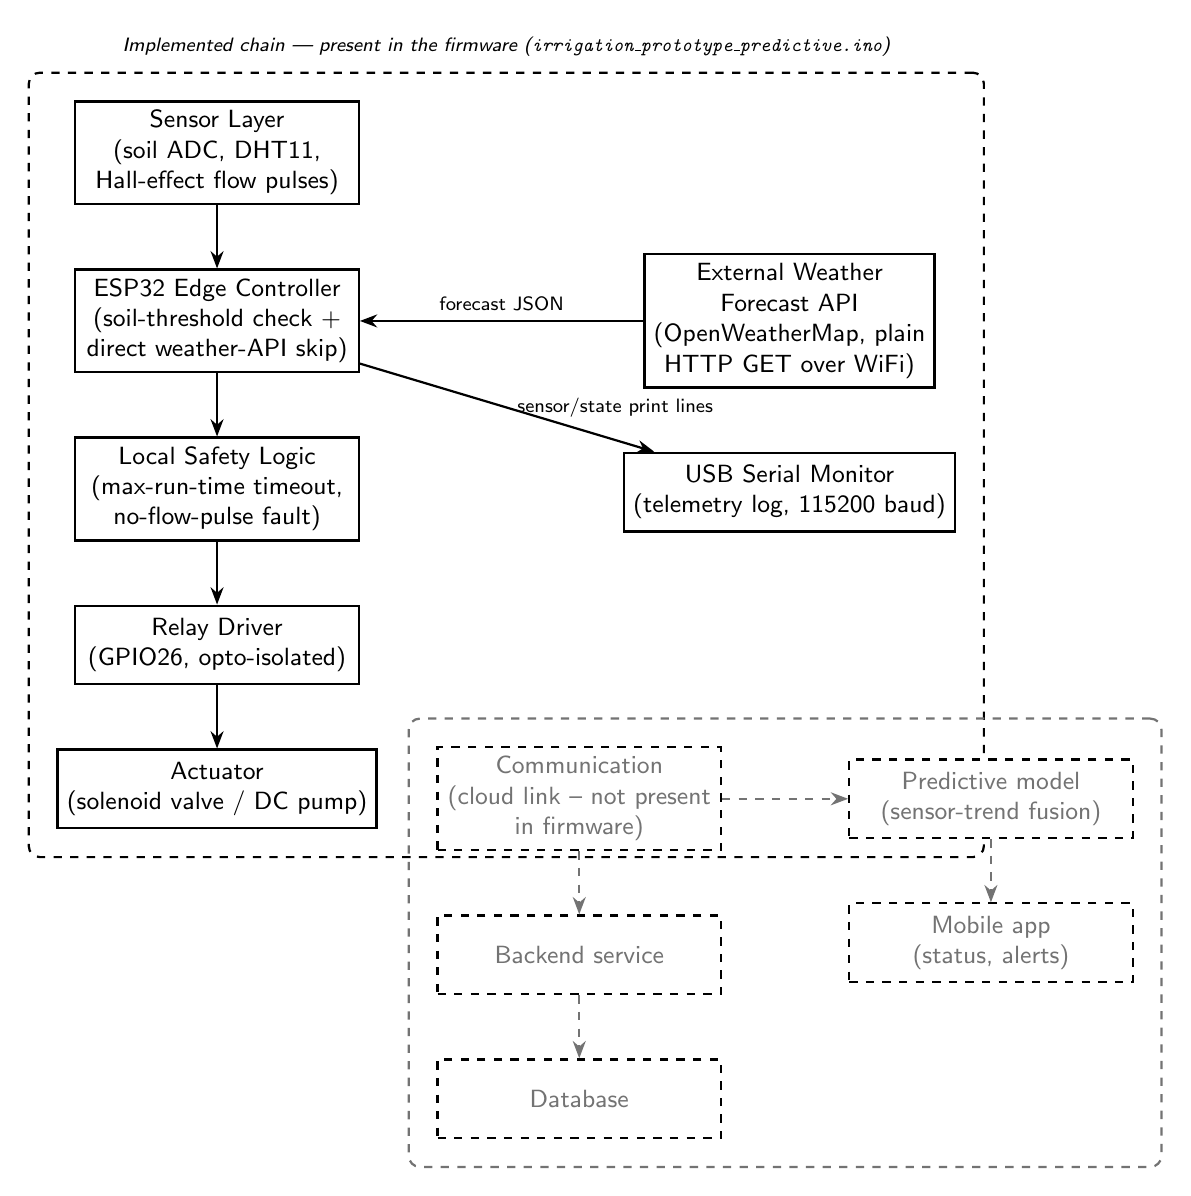
\begin{tikzpicture}[
  font=\sffamily\small,
  box/.style={draw, thick, rectangle, minimum width=3.6cm, minimum height=1cm, align=center, fill=white},
  propbox/.style={draw, thick, dashed, rectangle, minimum width=3.6cm, minimum height=1cm, align=center, fill=white, text=black!55},
  arr/.style={-{Stealth[length=2.2mm]}, thick},
  proparr/.style={-{Stealth[length=2.2mm]}, thick, dashed, draw=black!55},
  dashedbox/.style={draw, thick, dashed, inner sep=10pt, rounded corners}
]

% =====================================================================
% IMPLEMENTED CHAIN -- matches irrigation_prototype_predictive.ino
% =====================================================================
\node[box] (sensors) {Sensor Layer\\(soil ADC, DHT11,\\Hall-effect flow pulses)};
\node[box, below=0.8cm of sensors] (esp32) {ESP32 Edge Controller\\(soil-threshold check +\\direct weather-API skip)};
\node[box, below=0.8cm of esp32] (safety) {Local Safety Logic\\(max-run-time timeout,\\no-flow-pulse fault)};
\node[box, below=0.8cm of safety] (driver) {Relay Driver\\(GPIO26, opto-isolated)};
\node[box, below=0.8cm of driver] (actuator) {Actuator\\(solenoid valve / DC pump)};

\draw[arr] (sensors) -- (esp32);
\draw[arr] (esp32) -- (safety);
\draw[arr] (safety) -- (driver);
\draw[arr] (driver) -- (actuator);

\node[box, right=3.6cm of esp32] (weather) {External Weather\\Forecast API\\(OpenWeatherMap, plain\\HTTP GET over WiFi)};
\draw[arr] (weather) -- (esp32) node[midway, above, font=\sffamily\scriptsize] {forecast JSON};

\node[box, below=0.8cm of weather] (serial) {USB Serial Monitor\\(telemetry log, 115200 baud)};
\draw[arr] (esp32) -- (serial) node[midway, right, font=\sffamily\scriptsize] {sensor/state print lines};

% =====================================================================
% PROPOSED / NOT-YET-IMPLEMENTED EXTENSION
% =====================================================================
\node[propbox, below=2.6cm of safety, xshift=4.6cm] (comm) {Communication\\(cloud link -- not present\\in firmware)};
\node[propbox, below=0.8cm of comm] (backend) {Backend service};
\node[propbox, below=0.8cm of backend] (db) {Database};
\node[propbox, right=1.6cm of comm] (predictor) {Predictive model\\(sensor-trend fusion)};
\node[propbox, below=0.8cm of predictor] (app) {Mobile app\\(status, alerts)};

\draw[proparr] (comm) -- (backend);
\draw[proparr] (backend) -- (db);
\draw[proparr] (comm) -- (predictor);
\draw[proparr] (predictor) -- (app);

\begin{scope}[on background layer]
\node[dashedbox, fit=(sensors)(actuator)(weather)(serial)] (localbox) {};
\node[font=\sffamily\scriptsize\itshape, align=left, above=2pt of localbox.north, anchor=south]
  {Implemented chain --- present in the firmware (\texttt{irrigation\_prototype\_predictive.ino})};
\node[dashedbox, draw=black!55, fit=(comm)(backend)(db)(predictor)(app)] (remotebox) {};
\end{scope}

\end{tikzpicture}%
}
\caption{System architecture, with the implemented local chain
separated from the proposed (not-yet-implemented) cloud extension
described in the project's design documents.}
\label{fig:arch}
\end{figure}

The implemented chain operates as a single fast loop on the ESP32: read
sensors, evaluate the local safety interlocks, evaluate the irrigation
decision (reactive threshold plus predictive weather skip), drive the
relay, and print a telemetry line to the USB serial console. No part of
this loop depends on network connectivity except the predictive-skip
feature itself, which fails open to reactive-only behaviour when WiFi
or the weather API is unavailable (Section~\ref{sec:firmware}).

\section{Hardware Design}
\label{sec:hardware}

The edge controller is an ESP32-WROOM-32 development board
\cite{espressif2023esp32}, chosen for its dual ADC/interrupt-capable
GPIO, built-in WiFi, and low unit cost. Table~\ref{tab:bom} lists the
components documented in the project's design report and build guide.
The last column states whether each component's presence in the
assembled prototype is supported by a photograph (Category~4 in the
evidence scheme of Section~\ref{sec:evidence}) or only by design
documentation (Category~1).

\begin{table}[t]
\caption{Hardware bill of materials and evidentiary basis}
\label{tab:bom}
\centering
\begin{tabular}{@{}p{0.27\columnwidth}p{0.31\columnwidth}p{0.32\columnwidth}@{}}
\toprule
\textbf{Component} & \textbf{Role} & \textbf{Confirmed by photo?} \\
\midrule
ESP32-WROOM-32 DevKit & Edge controller: acquisition, local decision, actuation & Yes \\
Capacitive soil-moisture sensor (labelled ``V2.0.0'') & Soil-moisture input, GPIO34 (ADC1) & Yes \\
DHT11 temperature/humidity sensor & Ambient temperature and humidity input, GPIO4 & Probable (blue module consistent with a DHT11; label not legible) \\
Hall-effect turbine flow sensor & Pulse counting for volumetric accounting, GPIO27 & Yes (exact part number not legible) \\
1-channel opto-isolated relay module & Driver stage, GPIO26 & Yes \\
Solenoid valve / small DC pump & Water-delivery actuator & Pump: yes (model not legible); valve: not visible \\
Separate DC supply, flyback diode, fuse & Actuator power and protection & Design document only \\
Audible alert (buzzer) & Optional status indication & Probable (round component consistent with a buzzer); pin, wiring and firmware not confirmed \\
\bottomrule
\end{tabular}
\end{table}

Figure~\ref{fig:circuit} shows the pin-level connections as specified
by the firmware's pin definitions and header comments. It is a design
schematic derived from the source code and build documentation, not a
traced photograph of the assembled board. The relay polarity, i.e.\
whether GPIO26 HIGH or LOW energises the relay coil on the module used,
has not been confirmed and is marked as such on the diagram.

\begin{figure}[t]
\centering
\resizebox{\columnwidth}{!}{%
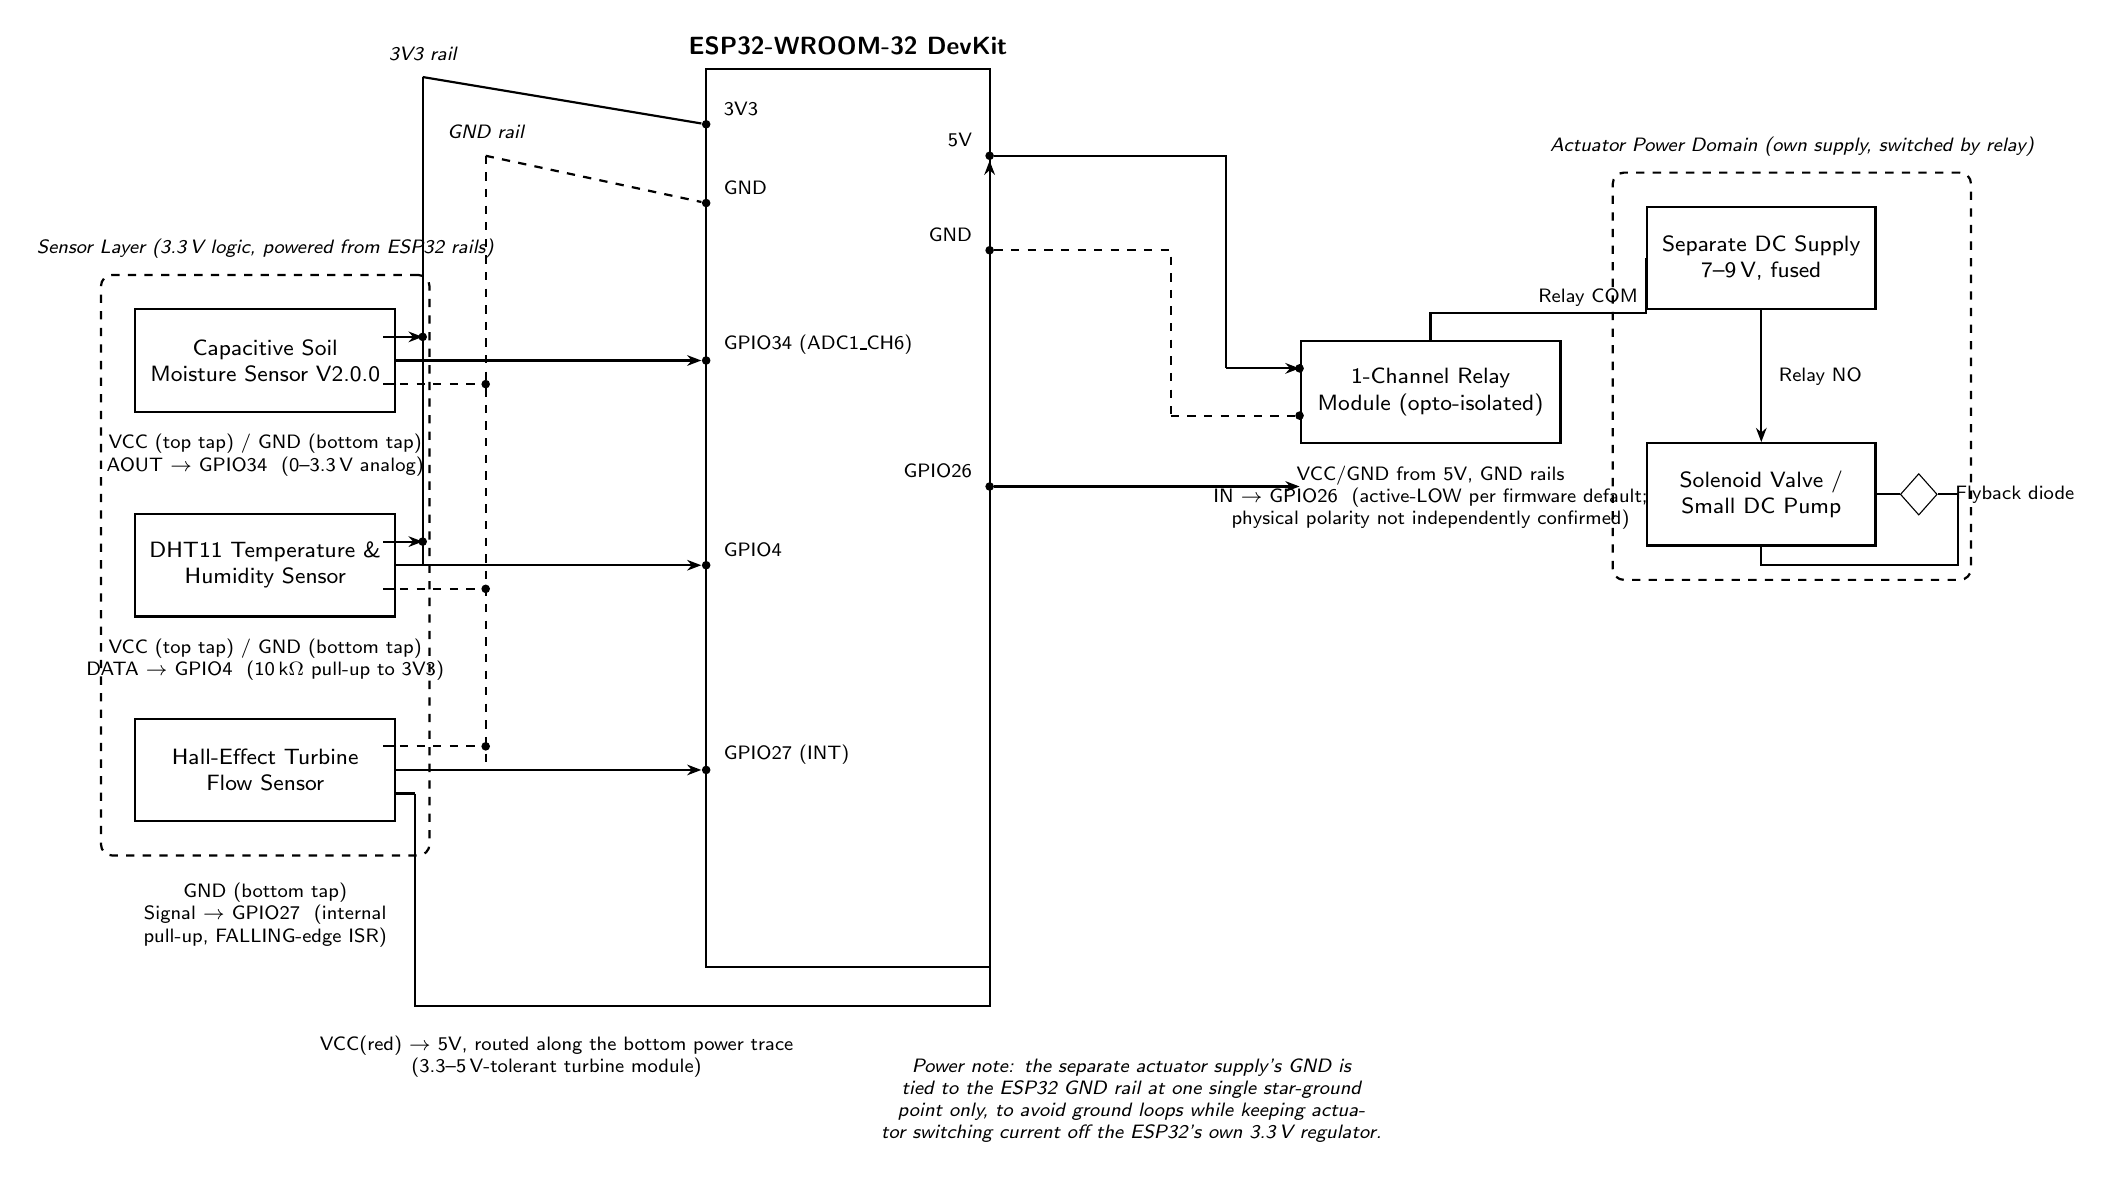
\begin{tikzpicture}[
  font=\sffamily\footnotesize,
  mcu/.style={draw, thick, rectangle, minimum width=3.6cm, minimum height=11.4cm, align=center, fill=white},
  dev/.style={draw, thick, rectangle, minimum width=3.3cm, minimum height=1.3cm, align=center, fill=white},
  pin/.style={font=\sffamily\scriptsize},
  raillbl/.style={font=\sffamily\scriptsize\itshape},
  wire/.style={thick},
  gndwire/.style={thick, dashed},
  arr/.style={-{Stealth[length=1.8mm]}, thick},
  junc/.style={circle, fill=black, inner sep=1.1pt}
]

% All coordinates are PLAIN (x,y) numbers in cm, chosen explicitly so every
% wire below is a single straight horizontal or vertical segment.

% ---- ESP32 body, centred at origin ----
\node[mcu] (esp) at (0,0) {};
\node[font=\sffamily\bfseries\small] at (0,6.0) {ESP32-WROOM-32 DevKit};

% ---- LEFT-edge pins (x = esp.west = -1.8) ----
\def\xL{-1.8}
\node[junc] (p3v3) at (\xL,5.0) {}; \node[pin, anchor=west] at (\xL+0.1,5.2) {3V3};
\node[junc] (pgndL) at (\xL,4.0) {}; \node[pin, anchor=west] at (\xL+0.1,4.2) {GND};
\node[junc] (p34)  at (\xL,2.0) {}; \node[pin, anchor=west] at (\xL+0.1,2.2) {GPIO34 (ADC1\_CH6)};
\node[junc] (p4)   at (\xL,-0.6) {}; \node[pin, anchor=west] at (\xL+0.1,-0.4) {GPIO4};
\node[junc] (p27)  at (\xL,-3.2) {}; \node[pin, anchor=west] at (\xL+0.1,-3.0) {GPIO27 (INT)};

% ---- RIGHT-edge pins (x = esp.east = 1.8) ----
\def\xR{1.8}
\node[junc] (p5v)  at (\xR,4.6) {}; \node[pin, anchor=east] at (\xR-0.1,4.8) {5V};
\node[junc] (pgndR) at (\xR,3.4) {}; \node[pin, anchor=east] at (\xR-0.1,3.6) {GND};
\node[junc] (p26)  at (\xR,0.4) {}; \node[pin, anchor=east] at (\xR-0.1,0.6) {GPIO26};

% =====================================================================
% LEFT SIDE: three sensors, each at the SAME y as its unique data pin
% =====================================================================
\node[dev] (soil) at (-7.4,2.0)  {Capacitive Soil\\Moisture Sensor V2.0.0};
\node[dev] (dht)  at (-7.4,-0.6) {DHT11 Temperature \&\\Humidity Sensor};
\node[dev] (flow) at (-7.4,-3.2) {Hall-Effect Turbine\\Flow Sensor};

% Bus rails: two vertical lines between sensors (x=-7.4) and MCU (x=-1.8)
\def\xVrail{-5.4}
\def\xGrail{-4.6}
\draw[wire]    (\xVrail,5.6) -- (\xVrail,-0.6);
\draw[wire]    (\xVrail,5.6) -- (p3v3);
\node[raillbl] at (\xVrail,5.9) {3V3 rail};

\draw[gndwire] (\xGrail,4.6) -- (\xGrail,-3.2);
\draw[gndwire] (\xGrail,4.6) -- (pgndL);
\node[raillbl] at (\xGrail,4.9) {GND rail};

% soil: VCC tap (upper stub), GND tap (lower stub), AOUT direct to GPIO34
\draw[wire,arr] (-5.9,2.3) -- (\xVrail,2.3) node[junc]{};
\draw[wire]     (soil.east |- 0,2.3) -- (-5.9,2.3);
\draw[gndwire]  (-5.9,1.7) -- (\xGrail,1.7) node[junc]{};
\draw[gndwire]  (soil.east |- 0,1.7) -- (-5.9,1.7);
\draw[wire,arr] (soil.east) -- (p34);
\node[pin, below=0.15cm of soil.south, align=center] {VCC (top tap) / GND (bottom tap)\\AOUT $\to$ GPIO34 \ (0--3.3\,V analog)};

% dht: VCC tap, GND tap, DATA direct to GPIO4
\draw[wire,arr] (-5.9,-0.3) -- (\xVrail,-0.3) node[junc]{};
\draw[wire]     (dht.east |- 0,-0.3) -- (-5.9,-0.3);
\draw[gndwire]  (-5.9,-0.9) -- (\xGrail,-0.9) node[junc]{};
\draw[gndwire]  (dht.east |- 0,-0.9) -- (-5.9,-0.9);
\draw[wire,arr] (dht.east) -- (p4);
\node[pin, below=0.15cm of dht.south, align=center] {VCC (top tap) / GND (bottom tap)\\DATA $\to$ GPIO4 \ (10\,k$\Omega$ pull-up to 3V3)};

% flow: GND tap to rail; Signal direct to GPIO27; VCC via bottom power trace to 5V
\draw[gndwire] (-5.9,-2.9) -- (\xGrail,-2.9) node[junc]{};
\draw[gndwire] (flow.east |- 0,-2.9) -- (-5.9,-2.9);
\draw[wire,arr] (flow.east) -- (p27);
\node[pin, below=0.65cm of flow.south, align=center, text width=3.3cm] {GND (bottom tap)\\Signal $\to$ GPIO27 \ (internal pull-up, FALLING-edge ISR)};

\draw[wire,arr] (-5.5,-3.5) -- (-5.5,-6.2) -- (\xR,-6.2) -- (p5v);
\draw[wire] (flow.east |- 0,-3.5) -- (-5.5,-3.5);
\node[pin, below=0.25cm of {(-3.7,-6.2)}, align=center] {VCC(red) $\to$ 5V, routed along the bottom power trace\\(3.3--5\,V-tolerant turbine module)};

% =====================================================================
% RIGHT SIDE: relay module and actuator power domain
% =====================================================================
\node[dev] (relay) at (7.4,1.6) {1-Channel Relay\\Module (opto-isolated)};

\def\xVrail2{4.8}
\def\xGrail2{4.1}
\draw[wire]    (p5v) -- (\xVrail2,4.6) -- (\xVrail2,1.9);
\draw[wire,arr] (\xVrail2,1.9) -- (relay.west |- 0,1.9) node[junc]{};
\draw[gndwire] (pgndR) -- (\xGrail2,3.4) -- (\xGrail2,1.3);
\draw[gndwire] (\xGrail2,1.3) -- (relay.west |- 0,1.3) node[junc]{};
\draw[wire,arr] (p26) -- (relay.west |- 0,0.4);
\node[pin, below=0.15cm of relay.south, align=center] {VCC/GND from 5V, GND rails\\IN $\to$ GPIO26 \ (active-LOW per firmware default;\\physical polarity not independently confirmed)};

\node[dev, minimum width=2.9cm] (psu) at (11.6,3.3) {Separate DC Supply\\7--9\,V, fused};
\node[dev, minimum width=2.9cm] (pump) at (11.6,0.3) {Solenoid Valve /\\Small DC Pump};

\draw[wire] (relay.north) -- (relay.north |- 0,2.6) -- (psu.west |- 0,2.6) -- (psu.west);
\node[pin] at (9.4,2.8) {Relay COM};
\draw[wire,arr] (psu.south) -- (pump.north);
\node[pin, right=0.1cm of {(11.6,1.8)}] {Relay NO};

\node[draw, diamond, minimum width=9pt, minimum height=15pt] (fd) at (13.6,0.3) {};
\draw[wire] (pump.east) -- (fd.west);
\draw[wire] (fd.east) -- (14.1,0.3) -- (14.1,-0.6) -- (11.6,-0.6) -- (pump.south);
\node[pin, right=0.1cm of fd] {Flyback diode};

% =====================================================================
% Power / grounding note
% =====================================================================
\node[pin, font=\sffamily\scriptsize\itshape, align=center, text width=8.0cm] at (3.6,-7.4)
  {Power note: the separate actuator supply's GND is tied to the ESP32 GND rail at one single star-ground point only, to avoid ground loops while keeping actuator switching current off the ESP32's own 3.3\,V regulator.};

\begin{scope}[on background layer]
\node[draw, dashed, thick, inner sep=12pt, rounded corners, fit=(soil)(dht)(flow)] (sensbox) {};
\node[font=\sffamily\scriptsize\itshape, above=2pt of sensbox.north] {Sensor Layer (3.3\,V logic, powered from ESP32 rails)};
\node[draw, dashed, thick, inner sep=12pt, rounded corners, fit=(psu)(pump)(fd)] (actbox) {};
\node[font=\sffamily\scriptsize\itshape, above=2pt of actbox.north] {Actuator Power Domain (own supply, switched by relay)};
\end{scope}

\end{tikzpicture}%
}
\caption{Pin-level circuit schematic derived from the firmware and
build documentation. This is a design diagram, not a photograph of the
assembled hardware.}
\label{fig:circuit}
\end{figure}

\ifshowphotos
Figure~\ref{fig:bench} shows the bench assembly. It contains the ESP32
development board, a capacitive soil-moisture sensor labelled ``V2.0.0'',
a yellow turbine-type flow sensor connected in-line with transparent
tubing, a one-channel relay module with illuminated indicator LEDs, and a
small pump connected to the same tubing. A blue module consistent with a
DHT11 sensor is visible beside the ESP32, and a small black round
component consistent with a buzzer is visible on the lower breadboard.
Neither of these two can be identified with certainty at the available
resolution, and their pin connections cannot be traced from the
photograph. Overall, the photograph indicates that the prototype was
assembled substantially as specified in the design documentation.

\begin{figure}[t]
\centering
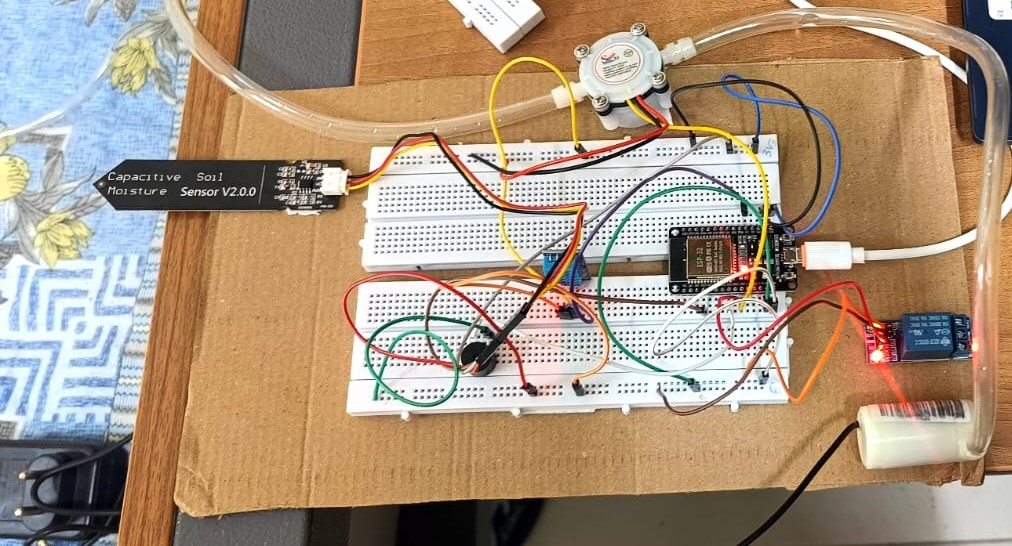
\includegraphics[width=\columnwidth]{figs/photo_bench.jpg}
\caption{Bench assembly of the prototype: ESP32 board, capacitive
soil-moisture sensor, Hall-effect flow sensor in-line with tubing, relay
module and a small pump.}
\label{fig:bench}
\end{figure}
\else
The prototype was assembled on a breadboard according to the schematic
in Fig.~\ref{fig:circuit}, using the components listed in
Table~\ref{tab:bom}. Photographs of the assembled hardware (not
reproduced here) are consistent with this configuration.

\fi

\section{Firmware and Control Logic}
\label{sec:firmware}

The firmware (\texttt{irrigation\_\allowbreak prototype\_\allowbreak predictive.ino}) is written against the
Arduino-ESP32 core \cite{espressif2024arduinocore} and depends on two
third-party libraries declared in its own header comments: the Adafruit
DHT sensor library \cite{adafruit2024dht} for the temperature/humidity
sensor, and ArduinoJson \cite{blanchon2024arduinojson} for parsing the
weather-API response. It implements the control flow in
Figure~\ref{fig:flow}. Four elements are described precisely below.

\begin{enumerate}
\item \textbf{Soil moisture} is read as a raw ADC value on GPIO34 and
linearly mapped to a 0--100\% scale using two calibration constants,
\texttt{SOIL\_DRY\_VALUE} and \texttt{SOIL\_WET\_VALUE}, which the
firmware's own comments mark as placeholders to be replaced with values
measured on the specific sensor unit used. Published studies of
low-cost capacitive soil-moisture sensors
\cite{adla2020laboratory,abdelmoneim2025calibration} describe
calibrating the sensor output against reference moisture measurements,
which is why a per-unit two-point calibration, not yet performed on this
prototype's sensor, is needed before \texttt{soilPct} can be treated as
an accurate percentage rather than a relative indicator.
\item \textbf{Volumetric flow} is computed by dividing the Hall-effect
sensor's pulse count by a calibration constant,
\texttt{FLOW\_CALIBRATION\_PULSES\_PER\_L}, which is likewise marked as
a placeholder (default value 450.0 pulses/L) pending a measured
calibration against a known poured volume (Section~\ref{sec:model}).
\item \textbf{The predictive skip} fires only when \texttt{soilPct} is
below the dry threshold \emph{and} the most recent OpenWeatherMap
forecast's probability-of-precipitation field exceeds a configurable
threshold (default 0.40); if the WiFi connection or the API call has
never succeeded, the system falls back to reactive-only behaviour by
design, rather than blocking irrigation on an unavailable forecast.
\item \textbf{Relay polarity} is controlled by a single boolean,
\texttt{RELAY\_ACTIVE\_LOW}, set to \texttt{true} by default; the
source comment directly above it reads ``VERIFY WITH YOUR OWN MODULE'',
i.e. the firmware's own author flagged this value as unverified at the
time of writing. It is therefore treated here as an open item rather
than a tested result.
\end{enumerate}

\begin{figure}[t]
\centering
\resizebox{\columnwidth}{!}{%
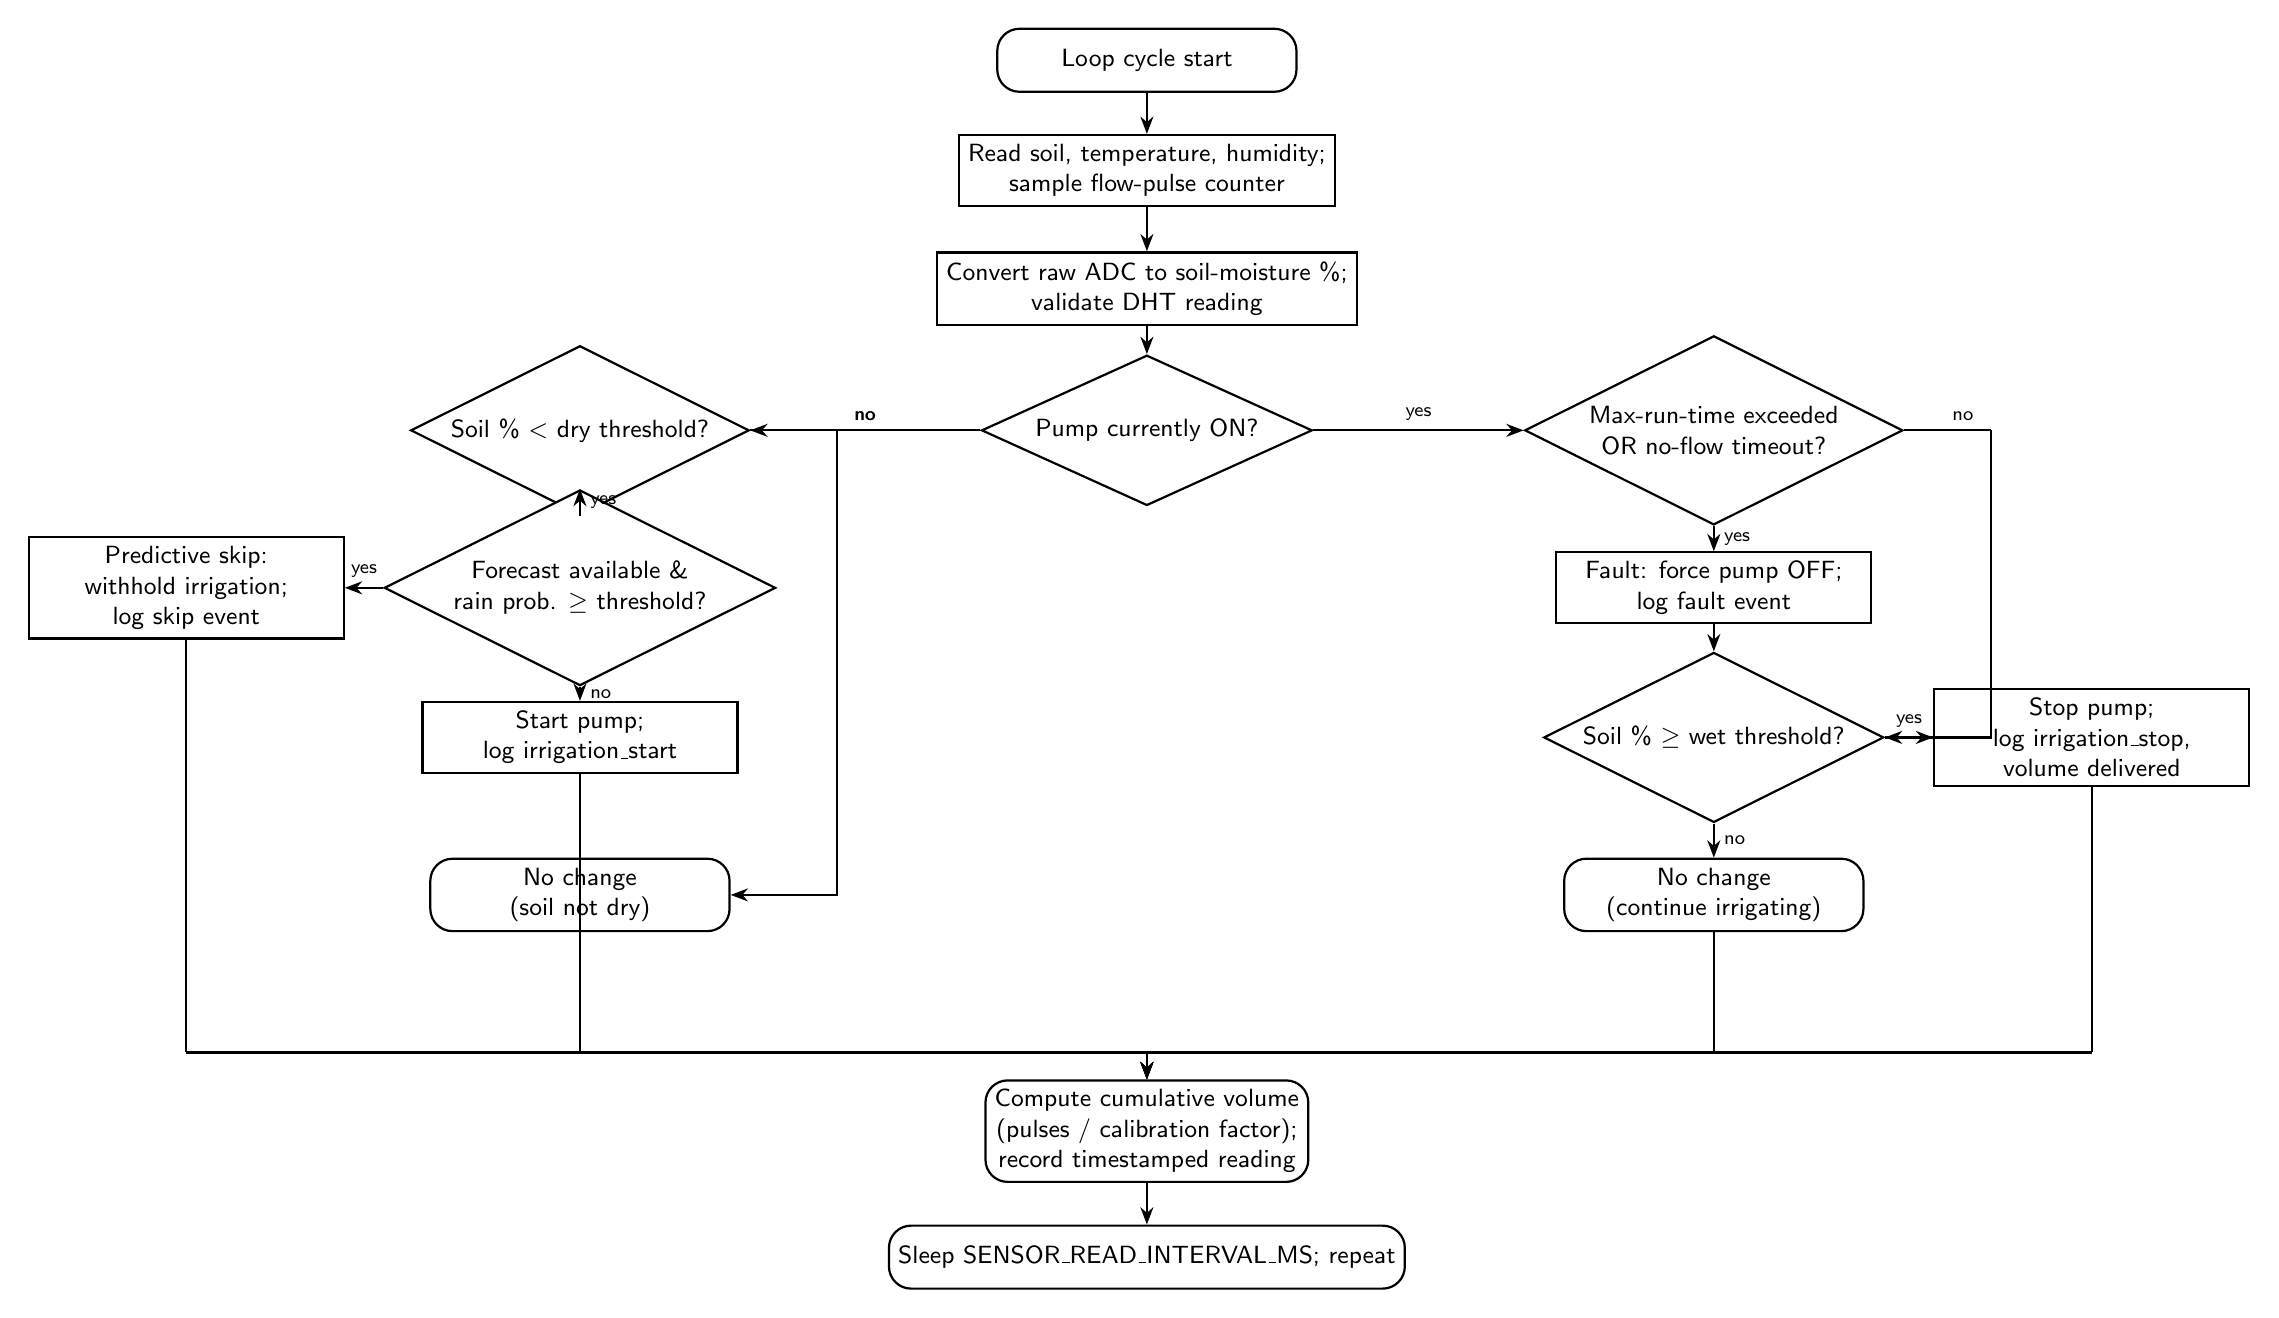
\begin{tikzpicture}[
  font=\sffamily\small,
  proc/.style={draw, thick, rectangle, minimum width=4.0cm, minimum height=0.9cm, align=center, fill=white},
  dec/.style={draw, thick, diamond, aspect=2.0, minimum width=4.2cm, minimum height=1.4cm, align=center, fill=white, inner sep=2pt},
  term/.style={draw, thick, rounded corners=8pt, minimum width=3.8cm, minimum height=0.8cm, align=center, fill=white},
  small/.style={font=\sffamily\scriptsize},
  arr/.style={-{Stealth[length=2.2mm]}, thick},
]

% ================= Shared spine (top) =================
\node[term] (start)   at (0,9.6)  {Loop cycle start};
\node[proc] (read)    at (0,8.2)  {Read soil, temperature, humidity;\\sample flow-pulse counter};
\node[proc] (convert) at (0,6.7)  {Convert raw ADC to soil-moisture \%;\\validate DHT reading};
\node[dec]  (pumpon)  at (0,4.9)  {Pump currently ON?};

\draw[arr] (start) -- (read);
\draw[arr] (read) -- (convert);
\draw[arr] (convert) -- (pumpon);

% ================= RIGHT branch: pump was ON =================
\node[dec]  (fault)     at (7.2,4.9)  {Max-run-time exceeded\\OR no-flow timeout?};
\node[proc] (faultstop) at (7.2,2.9)  {Fault: force pump OFF;\\log fault event};
\node[dec]  (wet)       at (7.2,1.0)  {Soil \% $\geq$ wet threshold?};
\node[proc] (stopon)    at (12.0,1.0) {Stop pump;\\log irrigation\_stop,\\volume delivered};
\node[term] (keepon)    at (7.2,-1.0) {No change\\(continue irrigating)};

\draw[arr] (pumpon.east) -- node[above,small]{yes} (fault.west);
\draw[arr] (fault.south) -- node[right,small]{yes} (faultstop.north);
\draw[arr] (faultstop.south) -- (wet.north);
\draw[thick] (fault.east) -- ++(1.1,0) coordinate (faultbypass);
\draw[arr]  (faultbypass) node[above,small,xshift=-10pt]{no} -- (faultbypass |- wet.east) -- (wet.east);
\draw[arr] (wet.east) -- node[above,small]{yes} (stopon.west);
\draw[arr] (wet.south) -- node[right,small]{no} (keepon.north);

% ================= LEFT branch: pump was OFF =================
\node[dec]  (dry)   at (-7.2,4.9)  {Soil \% $<$ dry threshold?};
\node[dec]  (rain)  at (-7.2,2.9)  {Forecast available \&\\rain prob. $\geq$ threshold?};
\node[proc] (skip)  at (-12.2,2.9) {Predictive skip:\\withhold irrigation;\\log skip event};
\node[proc] (starton) at (-7.2,1.0) {Start pump;\\log irrigation\_start};
\node[term] (nodecision) at (-7.2,-1.0) {No change\\(soil not dry)};

\draw[arr] (pumpon.west) -- node[above,small]{no} (dry.east);
\draw[thick] (dry.east) -- ++(1.1,0) coordinate (drybypass);
\draw[arr]  (drybypass) node[above,small,xshift=10pt]{no} -- (drybypass |- nodecision.east) -- (nodecision.east);
\draw[arr] (dry.south) -- node[right,small]{yes} (rain.north);
\draw[arr] (rain.west) -- node[above,small]{yes} (skip.east);
\draw[arr] (rain.south) -- node[right,small]{no} (starton.north);

% ================= Merge: all outcomes converge on logging =================
\node[term] (logall) at (0,-4.0) {Compute cumulative volume\\(pulses / calibration factor);\\record timestamped reading};

\def\collect{-3.0}
\draw[thick] (skip.south)       -- (skip.south |- 0,\collect);
\draw[thick] (starton.south)    -- (starton.south |- 0,\collect);
\draw[thick] (nodecision.south) -- (nodecision.south |- 0,\collect);
\draw[thick] (keepon.south)     -- (keepon.south |- 0,\collect);
\draw[thick] (stopon.south)     -- (stopon.south |- 0,\collect);
\draw[arr] (skip.south |- 0,\collect)       -- (0,\collect) -- (logall.north);
\draw[arr] (starton.south |- 0,\collect)    -- (0,\collect) -- (logall.north);
\draw[arr] (nodecision.south |- 0,\collect) -- (0,\collect) -- (logall.north);
\draw[arr] (keepon.south |- 0,\collect)     -- (0,\collect) -- (logall.north);
\draw[arr] (stopon.south |- 0,\collect)     -- (0,\collect) -- (logall.north);

\node[term] (endloop) at (0,-5.6) {Sleep SENSOR\_READ\_INTERVAL\_MS; repeat};
\draw[arr] (logall) -- (endloop);

\end{tikzpicture}%
}
\caption{Control flow of the main loop, reconstructed from the firmware.}
\label{fig:flow}
\end{figure}

Algorithm~\ref{alg:decide} restates the irrigation-decision function in
pseudocode, matching the source in its conditional structure.

\begin{algorithm}[t]
\caption{Irrigation decision (as implemented)}
\label{alg:decide}
\begin{algorithmic}[1]
\IF{pump is OFF}
  \IF{soilPct $<$ SOIL\_DRY\_THRESHOLD\_PCT}
    \IF{weatherAvailable \AND rainExpected}
      \STATE log ``predictive skip''; leave pump OFF
    \ELSE
      \STATE turn pump ON
    \ENDIF
  \ENDIF
\ELSE
  \IF{soilPct $\geq$ SOIL\_WET\_THRESHOLD\_PCT}
    \STATE turn pump OFF
  \ENDIF
\ENDIF
\STATE \COMMENT{evaluated every loop, independent of the above:}
\IF{pump is ON \AND (run-time $>$ MAX\_PUMP\_RUN\_MS \OR no new pulses for $>$ NO\_FLOW\_GRACE\_MS)}
  \STATE force pump OFF; log fault
\ENDIF
\end{algorithmic}
\end{algorithm}

\section{Water-Balance Model}
\label{sec:model}

The Hall-effect turbine sensor produces output pulses at a rate
approximately proportional to the instantaneous volumetric flow rate
$Q$, so that the delivered volume over an irrigation event is
\begin{equation}
V = \frac{N}{K}
\label{eq:volume}
\end{equation}
where $N$ is the pulse count accumulated during the event (read from
the ESP32 interrupt-driven counter on GPIO27, falling-edge triggered)
and $K$ is an empirically-measured calibration constant, in pulses per
litre, obtained by passing a known volume through the sensor and
dividing the resulting pulse count by that volume. This is the formula
the firmware implements (\texttt{pulsesToLitres()}). An earlier reference
formula used during the design phase was dimensionally inconsistent and
was corrected before any hardware was built. Because the calibration
constant $K$ in the firmware is
still the placeholder value (450.0 pulses/L) rather than a value
measured on the specific sensor unit assembled, any volume figure the
current build would report should be treated as uncalibrated until that
measurement step is carried out and the constant is updated accordingly.
This direct, pulse-counted volumetric model is a deliberately simpler
alternative to standard reference-evapotranspiration-based scheduling
methods such as the FAO Penman--Monteith method \cite{allen1998fao56},
which estimate crop water demand from weather variables rather than
measuring delivered volume directly; the firmware does not implement an
evapotranspiration model of any kind.

\section{Evidentiary Classification}
\label{sec:evidence}

The project's supporting materials include both independently sourced
documents and content drafted during earlier design phases. Every
substantive claim in this paper is therefore classified into one of five
categories: (1)~design-phase information or code that has not been
independently verified; (2)~implementation steps confirmed by the student
team; (3)~outputs or observations recorded in project notes but not
reproducible from a file; (4)~primary evidence (a source file or
photograph); and (5)~claims that remain unverified. Table~\ref{tab:evidence}
applies this scheme to the main claims made, or declined, in this paper.

\begin{table}[t]
\caption{Evidentiary basis of the main claims in this paper}
\label{tab:evidence}
\centering
\begin{tabular}{@{}p{0.58\columnwidth}p{0.32\columnwidth}@{}}
\toprule
\textbf{Claim} & \textbf{Category} \\
\midrule
Pin map (GPIO34/4/27/26) and control logic described in Sections~\ref{sec:firmware}--\ref{sec:model} & 4 (firmware source file) \\
Physical assembly of ESP32, soil sensor, flow sensor, relay and pump on a breadboard & 4 (photograph) \\
Live sensor telemetry (temperature, humidity, soil raw value, zero flow pulses, relay OFF) on 1 Sept.\ 2026 & 4 (photograph of serial monitor) \\
Relay energises on GPIO26 LOW (active-LOW) & 5 --- unverified; firmware default only \\
Flow sensor is a specific YF-S201 or YF-S401 model & 5 --- unverified; generic Hall-effect turbine type confirmed, exact model not legible in available photo \\
A buzzer/audible alert was implemented on a specific GPIO pin & 5 --- a \texttt{beep()} function was visible in one photographed code screenshot of a differently named firmware file; the pin assignment, and whether this version was ever flashed, are unconfirmed \\
Physical hardware assembly was carried out by the student team & 2 (team-confirmed) \\
Water savings, prediction accuracy, calibration accuracy & 5 --- no quantitative test has been performed \\
\bottomrule
\end{tabular}
\end{table}

\section{Bench Observations}
\label{sec:observations}

The only run-time evidence available is a single
photograph of a laptop screen\ifshowphotos{} (Fig.~\ref{fig:serial})\fi, dated 1 September 2026, 10:29~PM,
showing the Arduino IDE serial monitor connected to an ESP32 over
\texttt{COM7} at 115200 baud. The logged lines show temperature
steady at 22.90\textdegree C, humidity in the range 63.2--63.3\%, a
soil reading reported as 100\% (raw ADC values 1171--1196, consistent
with the sensor being in a fully wet reference condition), flow pulses
at 0 throughout, the forecast-skip variable reporting ``Rain expected:
NO'', and the relay reporting ``OFF'' on every line. This is consistent
with a bench test under no active water flow, as also described in the
project's second review presentation. It demonstrates that
the sensor-acquisition and serial-telemetry path of some version of the
firmware executed on real hardware and produced live, internally
consistent multi-sensor readings; it does \emph{not} demonstrate pump
actuation, relay polarity, flow-sensor accuracy, or any outcome of the
predictive-skip logic under an actual rain event, none of which appear
in this or any other available material. The firmware file name visible
in that screenshot (\texttt{irrigation\_predictive\_combined.ino})
differs from the file described in Sections~\ref{sec:firmware}--\ref{sec:model}
(\texttt{irrigation\_prototype\_predictive.ino}); the two share the same
pin map and the same active-low ternary pattern in their relay-driving
function, but are not byte-identical, and the exact contents of the
version actually running in the photograph are not otherwise available
for inspection.

\ifshowphotos
\begin{figure}[t]
\centering
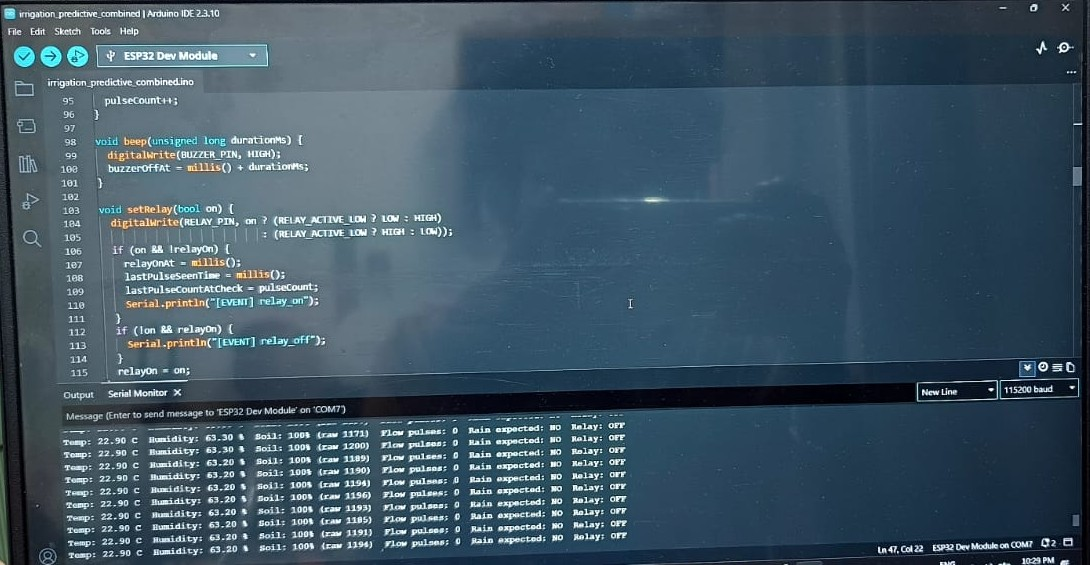
\includegraphics[width=\columnwidth]{figs/photo_serial.jpg}
\caption{Arduino IDE serial monitor during the bench test of 1 September
2026, showing live temperature, humidity, soil, flow-pulse, forecast and
relay fields.}
\label{fig:serial}
\end{figure}
\fi

\section{Limitations and Threats to Validity}
\label{sec:limitations}

This section lists the limits of the evidence presented in this paper.

\begin{itemize}
\item \textbf{No calibration has been performed.} Both calibration
constants used by the firmware (\texttt{SOIL\_DRY\_VALUE}/\texttt{SOIL\_WET\_VALUE}
and \texttt{FLOW\_CALIBRATION\_PULSES\_PER\_L}) remain at their
placeholder defaults in the firmware source file. Any moisture
percentage or volume figure the current build would output should be
treated as uncalibrated.
\item \textbf{Relay polarity is unverified.} The firmware defaults to
active-LOW and flags this for verification; an earlier project design
diagram assumed the opposite polarity. Neither has been checked against
the physical relay module, and this paper does not assert which is
correct.
\item \textbf{The flow-sensor model number is unconfirmed.} The sensor
visible in the photograph is a small Hall-effect turbine type
consistent with the YF-S* sensor family used in the project's build
guide, but its printed label is not legible at the resolution available,
and two different model numbers appear across the project's own
documents.
\item \textbf{Buzzer/alert hardware is not confirmed as implemented or
tested.} A \texttt{beep()} function is visible in one photographed code
screenshot, and a component consistent with a buzzer appears in the bench
photograph, but the function belongs to a firmware file whose full contents
are not available, so neither the GPIO assignment, nor the wiring, nor
whether the alert was ever exercised on hardware can be stated with
confidence.
\item \textbf{No water-balance, prediction-accuracy, or water-saving
results exist.} The project's own design report explicitly places any
claim of measured water savings, sensor accuracy, or predictive-model
performance out of scope for the design phase it documents, and no
later material supplies such a measurement.
This paper accordingly reports implementation status rather than
experimental results.
\item \textbf{Single-sample bench evidence.} The one serial-monitor
observation in Section~\ref{sec:observations} is a single time point
under static, no-flow conditions and should not be read as a
repeated or statistically meaningful test.
\end{itemize}

The additional tests that would be needed to move the corresponding
claims from ``unverified'' to ``verified'' are, respectively: a
multimeter or oscilloscope check of the relay coil's drive state at
each GPIO26 level; a legible photograph or purchase record of the flow
sensor's printed label; the source file and a hardware test of whichever
firmware version actually contains the \texttt{beep()} function; and a
controlled calibration procedure (known-volume pours for the flow
sensor, open-air/submerged readings for the soil sensor) followed by an
irrigation run with before/after soil-moisture logging.

\section{Conclusion and Future Work}
\label{sec:conclusion}

This paper has presented the design and current bench-implementation
status of an ESP32-based predictive drip-irrigation controller that
combines local soil-moisture thresholding with a direct weather-forecast
check and two independent safety interlocks. The evidence classification
in Table~\ref{tab:evidence} separates design diagrams, observed behaviour
and unverified claims, and can be reused in other early-stage hardware
projects whose documentation outpaces their verified results.

Future work, in priority order, is: (i)~perform and record the two
outstanding sensor calibrations; (ii)~confirm relay polarity against
the physical module and correct whichever of the firmware default or
the design diagram is wrong; (iii)~run a controlled irrigation cycle
with before/after soil-moisture and delivered-volume logging to produce
the first quantitative results; and (iv)~only once
local behaviour is validated, implement the proposed cloud extension
(Fig.~\ref{fig:arch}, lower half).

\section*{Acknowledgment}
The authors thank the project supervisor for guidance during the design
phase of the project.

\begin{thebibliography}{00}
\bibitem{gutierrez2014automated} J.~Guti\'{e}rrez, J.~F.~Villa-Medina, A.~Nieto-Garibay, and M.~\'{A}.~Porta-G\'{a}ndara, ``Automated irrigation system using a wireless sensor network and GPRS module,'' \emph{IEEE Trans. Instrum. Meas.}, vol.~63, no.~1, pp.~166--176, Jan. 2014, doi: 10.1109/TIM.2013.2276487.

\bibitem{kamienski2019smart} C.~Kamienski \emph{et al.}, ``Smart water management platform: IoT-based precision irrigation for agriculture,'' \emph{Sensors}, vol.~19, no.~2, p.~276, 2019, doi: 10.3390/s19020276.

\bibitem{vaishali2017mobile} S.~Vaishali, S.~Suraj, G.~Vignesh, S.~Dhivya, and S.~Udhayakumar, ``Mobile integrated smart irrigation management and monitoring system using IOT,'' in \emph{Proc. 2017 Int. Conf. Commun. Signal Process. (ICCSP)}, 2017, doi: 10.1109/ICCSP.2017.8286792.

\bibitem{jha2019comprehensive} K.~Jha, A.~Doshi, P.~Patel, and M.~Shah, ``A comprehensive review on automation in agriculture using artificial intelligence,'' \emph{Artif. Intell. Agric.}, vol.~2, pp.~1--12, 2019, doi: 10.1016/j.aiia.2019.05.004.

\bibitem{garcia2020iot} L.~Garc\'{i}a, L.~Parra, J.~M.~Jimenez, J.~Lloret, and P.~Lorenz, ``IoT-based smart irrigation systems: An overview on the recent trends on sensors and IoT systems for irrigation in precision agriculture,'' \emph{Sensors}, vol.~20, no.~4, p.~1042, 2020, doi: 10.3390/s20041042.

\bibitem{ferrandez2018precision} F.~J.~Ferr\'{a}ndez-Pastor, J.~M.~Garc\'{i}a-Chamizo, M.~Nieto-Hidalgo, and J.~Mora-Mart\'{i}nez, ``Precision agriculture design method using a distributed computing architecture on internet of things context,'' \emph{Sensors}, vol.~18, no.~6, p.~1731, 2018, doi: 10.3390/s18061731.

\bibitem{krizanovic2023lora} V.~Kri\v{z}anovi\'{c}, K.~Grgi\'{c}, J.~Spi\v{s}i\'{c}, and D.~\v{Z}agar, ``An advanced energy-efficient environmental monitoring in precision agriculture using LoRa-based wireless sensor networks,'' \emph{Sensors}, vol.~23, no.~14, p.~6332, 2023, doi: 10.3390/s23146332.

\bibitem{abdelmoneim2025calibration} A.~A.~Abdelmoneim, C.~M.~Al Kalaany, R.~Khadra, B.~Derardja, and G.~Dragonetti, ``Calibration of low-cost capacitive soil moisture sensors for irrigation management applications,'' \emph{Sensors}, vol.~25, no.~2, p.~343, 2025, doi: 10.3390/s25020343.

\bibitem{adla2020laboratory} S.~Adla, N.~K.~Rai, S.~H.~Karumanchi, S.~Tripathi, M.~Disse, and S.~Pande, ``Laboratory calibration and performance evaluation of low-cost capacitive and very low-cost resistive soil moisture sensors,'' \emph{Sensors}, vol.~20, no.~2, p.~363, 2020, doi: 10.3390/s20020363.

\bibitem{niti2019cwmi} NITI Aayog, Government of India, ``Composite water management index 2.0,'' NITI Aayog, New Delhi, India, Tech. Rep., 2019. [Online]. Available: \url{https://www.niti.gov.in/sites/default/files/2023-03/Composite%20Water%20Management%20Index%202.0.pdf}

\bibitem{fao2024aquastat} Food and Agriculture Organization of the United Nations, ``AQUASTAT country profile --- India,'' FAO AQUASTAT Global Information System on Water and Agriculture, 2024. [Online]. Available: \url{https://www.fao.org/aquastat/en/geospatial-information/global-maps-irrigated-areas/irrigation-by-country/country/IND}

\bibitem{rodell2009groundwater} M.~Rodell, I.~Velicogna, and J.~S.~Famiglietti, ``Satellite-based estimates of groundwater depletion in India,'' \emph{Nature}, vol.~460, no.~7258, pp.~999--1002, Aug. 2009, doi: 10.1038/nature08238.

\bibitem{allen1998fao56} R.~G.~Allen, L.~S.~Pereira, D.~Raes, and M.~Smith, \emph{Crop Evapotranspiration --- Guidelines for Computing Crop Water Requirements}, FAO Irrigation and Drainage Paper 56. Rome, Italy: Food and Agriculture Organization of the United Nations, 1998.

\bibitem{espressif2023esp32} Espressif Systems, \emph{ESP32 Technical Reference Manual}, 2023. [Online]. Available: \url{https://www.espressif.com/sites/default/files/documentation/esp32_technical_reference_manual_en.pdf}

\bibitem{owm2024forecast} OpenWeather Ltd., ``5 day / 3 hour forecast API documentation,'' OpenWeatherMap, 2024. [Online]. Available: \url{https://openweathermap.org/forecast5}

\bibitem{adafruit2024dht} Adafruit Industries, ``DHT sensor library (Arduino),'' GitHub repository, 2024. [Online]. Available: \url{https://github.com/adafruit/DHT-sensor-library}

\bibitem{blanchon2024arduinojson} B.~Blanchon, ``ArduinoJson,'' 2024. [Online]. Available: https://arduinojson.org

\bibitem{espressif2024arduinocore} Espressif Systems, ``Arduino core for the ESP32,'' GitHub repository, 2024. [Online]. Available: \url{https://github.com/espressif/arduino-esp32}

\bibitem{tzounis2017iot} A.~Tzounis, N.~Katsoulas, T.~Bartzanas, and C.~Kittas, ``Internet of Things in agriculture, recent advances and future challenges,'' \emph{Biosyst. Eng.}, vol.~164, pp.~31--48, Dec. 2017.

\bibitem{verdouw2016iot} C.~Verdouw, S.~Wolfert, and B.~Tekinerdogan, ``Internet of Things in agriculture,'' \emph{CAB Rev.}, vol.~11, no.~035, pp.~1--12, 2016, doi: 10.1079/PAVSNNR201611035.

\end{thebibliography}

\end{document}
